\section{Interface}
\label{sect:kegg_interface}

\begin{figure}
    \center{
        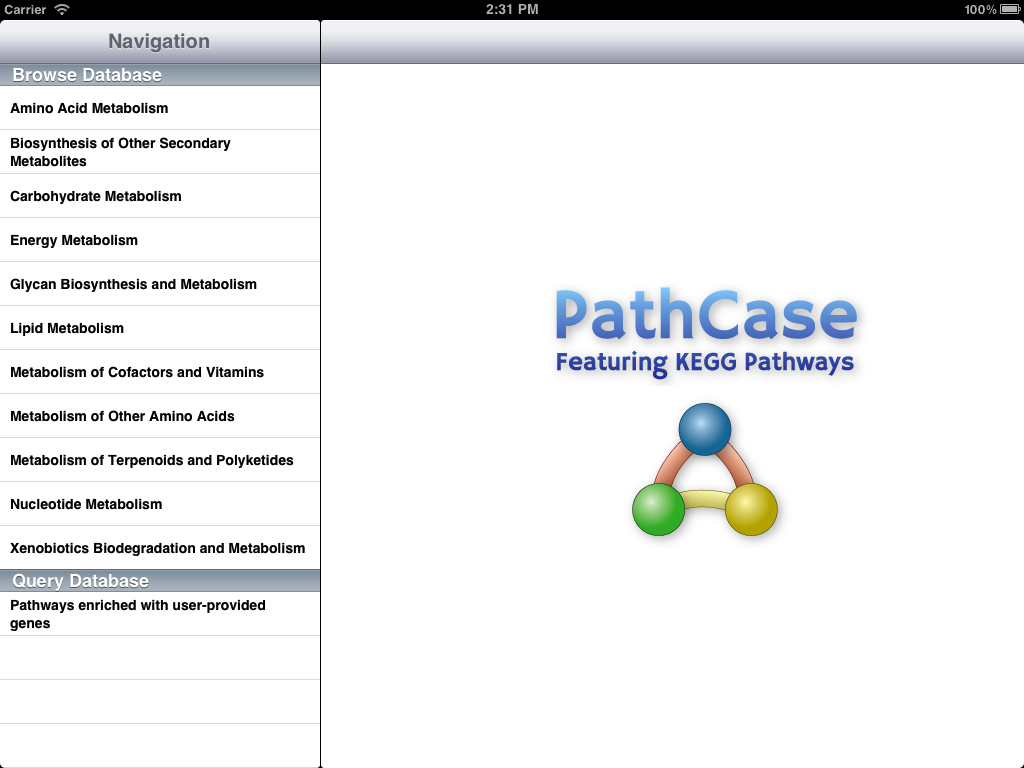
\includegraphics[width=3in]{kegg/figures/screenshot_list}}
    \caption{\label{fig:kegg_screenshot_list} List of pathway categories on
    the main screen of the KEGG app}
\end{figure}

\begin{figure}
    \center{
        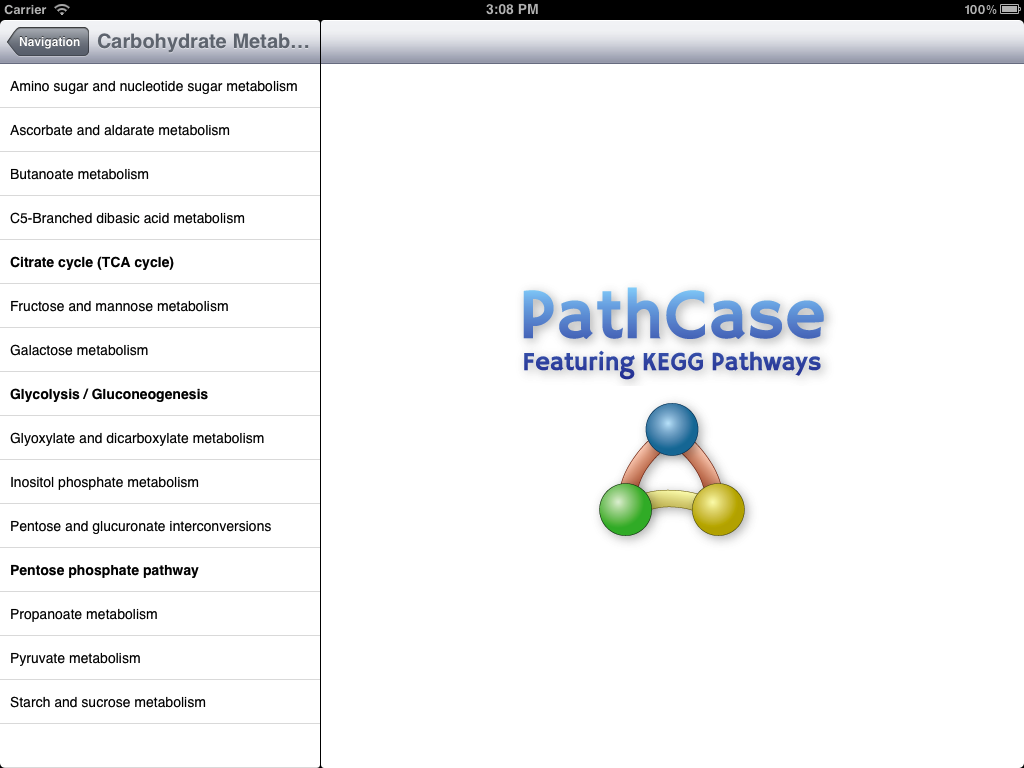
\includegraphics[width=3in]{kegg/figures/screenshot_sublist}}
    \caption{\label{fig:kegg_screenshot_sublist} List of pathways in the
    ``Carbohydrate Metabolism'' category of the KEGG app}
\end{figure}

The home screen of the KEGG app displays a list of pathway categories. Selecting
a category takes the user to a list of pathways. These lists are shown in
figures \ref{fig:kegg_screenshot_pathway} and \ref{fig:kegg_screenshot_sublist}.

After selecting a pathway, the user enters the graph view, where they can pan
and zoom across a pathway. The view for the TCA cycle is shown in figure
\ref{fig:kegg_screenshot_pathway}.

\begin{figure}[hbt]
    \center{
        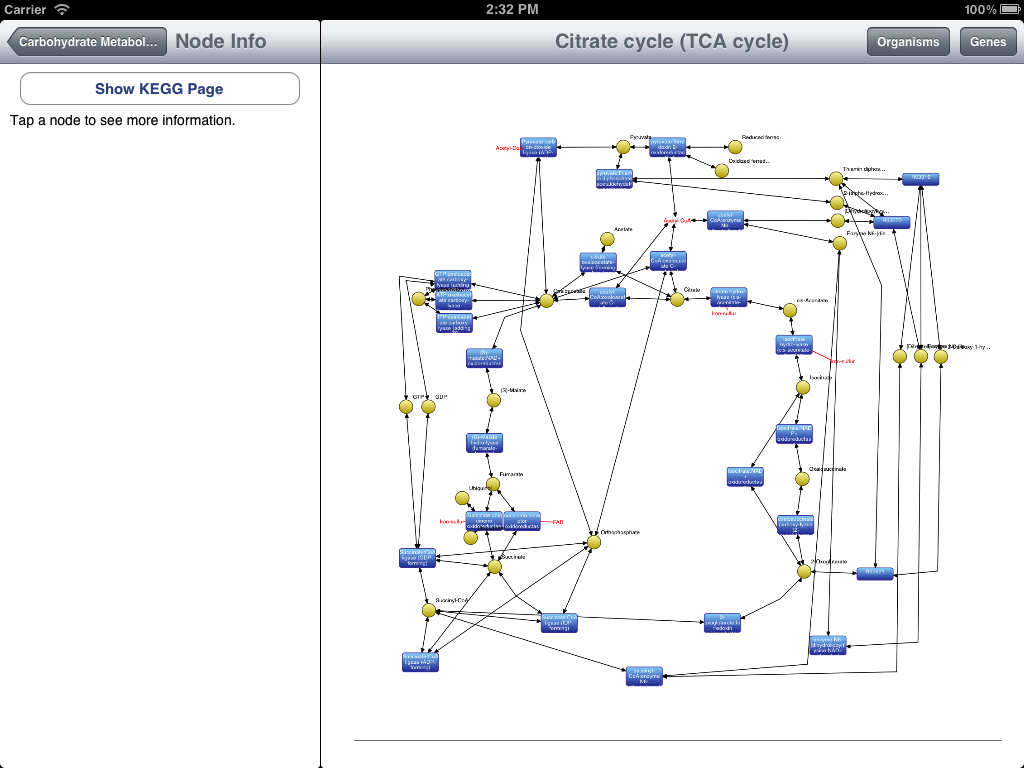
\includegraphics[width=3in]{kegg/figures/screenshot_pathway}}
    \caption{\label{fig:kegg_screenshot_pathway} Scrolling, zooming view of
    the TCA cycle}
\end{figure}


The graph view differs from the MAW app's graph view in several ways. The first
is the presence of the sidebar, which displays information about the user's
current selection. If no node is selected, it displays a button to show the KEGG
database web page for the pathway. (One example page is shown in figure
\ref{fig:kegg_screenshot_kegg_web_site}.

\begin{figure}[hbt]
    \center{
        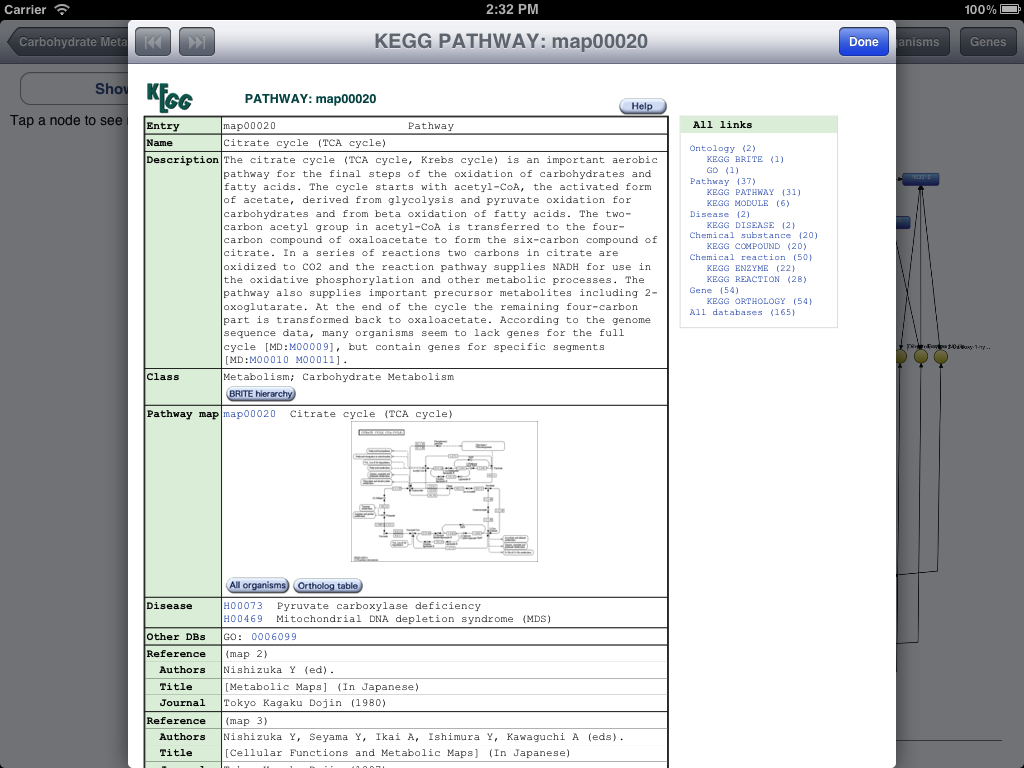
\includegraphics[width=3in]{kegg/figures/screenshot_kegg_web_site}}
    \caption{\label{fig:kegg_screenshot_kegg_web_site} KEGG web page for the TCA
    cycle, displayed by tapping the sidebar button}
\end{figure}

If the user taps a node, the sidebar shows a longer description of the node.
This differs from the MAW app behavior of using a popover to display the longer
description. Figure \ref{fig:kegg_screnshot_selection_no_info}

\begin{figure}[hbt]
    \center{
        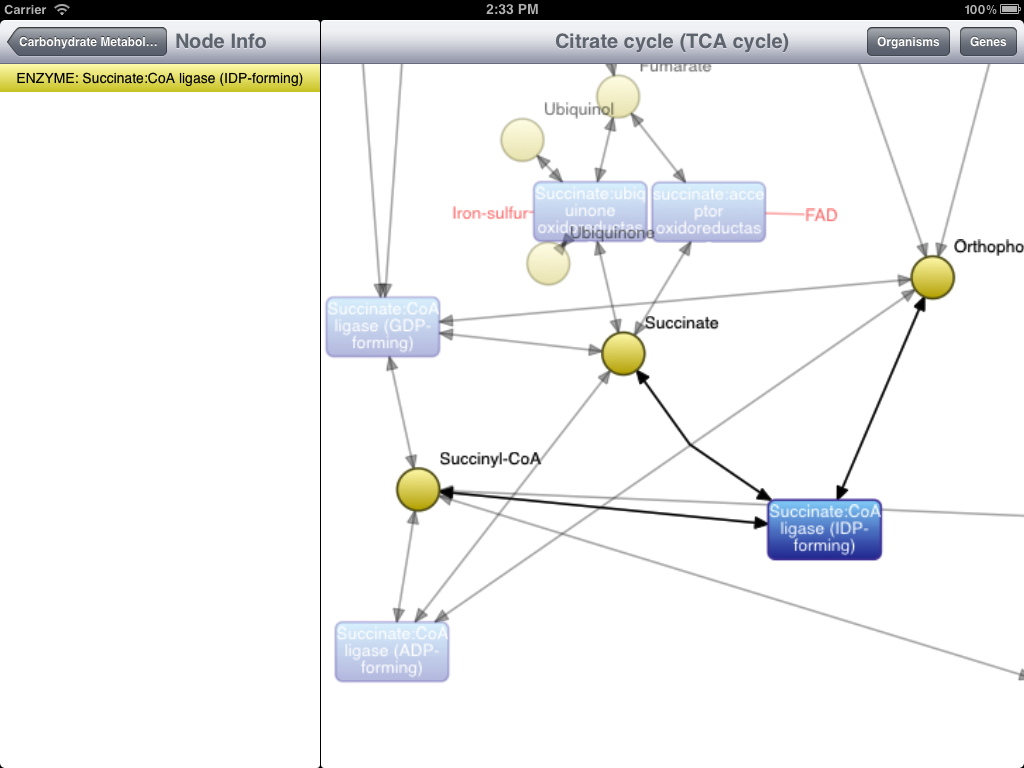
\includegraphics[width=3in]{kegg/figures/screenshot_selection_no_info}}
    \caption{\label{fig:kegg_screenshot_selection_no_info} Sidebar showing
    long description of a node in the KEGG app}
\end{figure}

The second major difference is the addition of the ``Organisms'' button in the
upper right corner. This button triggers a popover which allows the user to
activate and deactivate organisms. If a reaction is not present in any activated
organism, it is made partially transparent.

The organism hierarchy menu is shown in figure
\ref{fig:kegg_screenshot_animals_only_list}. The graph view corresponding to the
selection is shown in figure \ref{fig:kegg_screenshot_animals_only_graph}.

\begin{figure}[hbt]
    \center{
        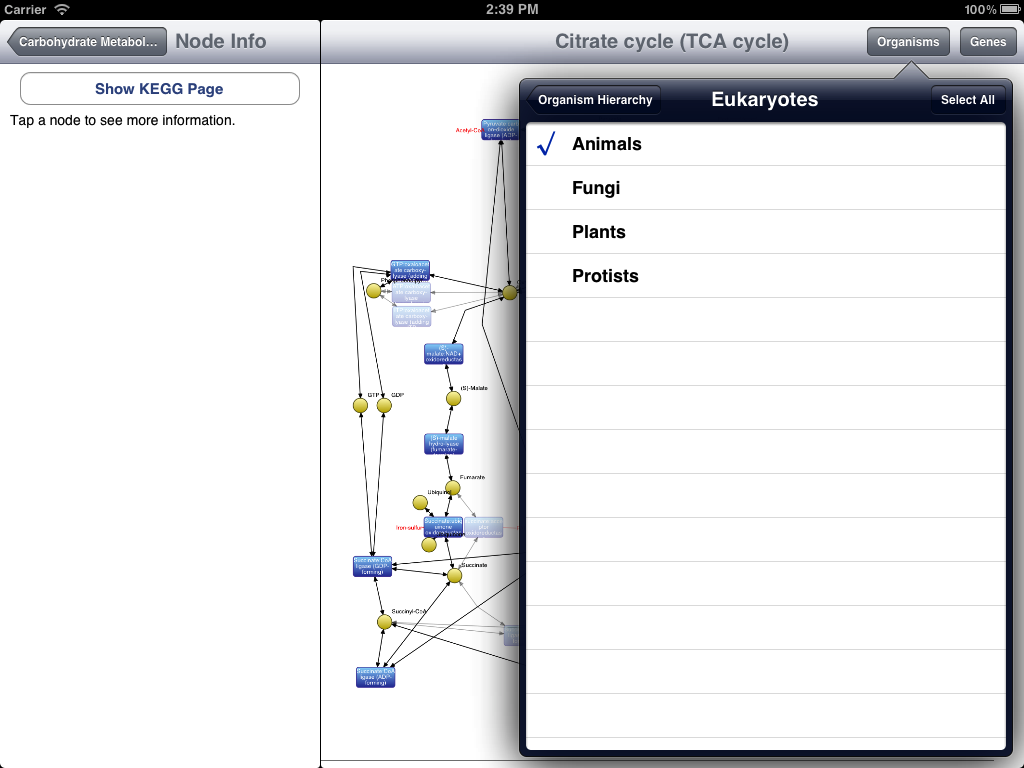
\includegraphics[width=3in]{kegg/figures/screenshot_animals_only_list}}
    \caption{\label{fig:kegg_screenshot_animals_only_list} Organism hierarchy
    menu with only Eukaryotes $\rightarrow$ Animals activated}
\end{figure}

\begin{figure}[hbt]
    \center{
        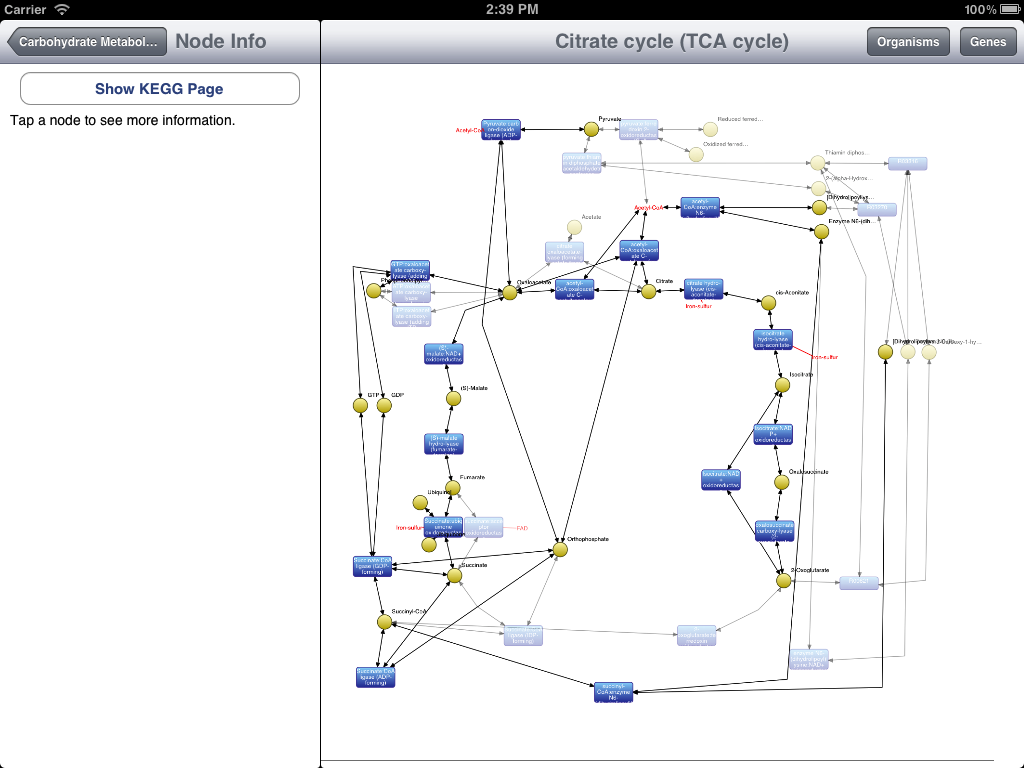
\includegraphics[width=3in]{kegg/figures/screenshot_animals_only_graph}}
    \caption{\label{fig:kegg_screenshot_animals_only_graph} Graph view with only
    reactions for Eukaryotes $\rightarrow$ Animals activated}
\end{figure}

\subsection{ENZYME Database Information}

%screenshot_selection_info.png

In addition to displaying a node's long description from PathCase KEGG, the KEGG
iPad app uses data from the ENZYME enzyme nomenclature database to show more
information for reactions for which EC numbers are available.

ENZYME's data comes from the recommendations of the Nomenclature Committee of
the International Union of Biochemistry and Molecular Biology (IUBMB)
\cite{enzyme-database}. An example of ENZYME information in the sidebar is shown
in figure \ref{fig:kegg_screenshot_selection_info}, including alternate names,
catalytic activity, cofactors, and more.

\begin{figure}[hbt]
    \center{
        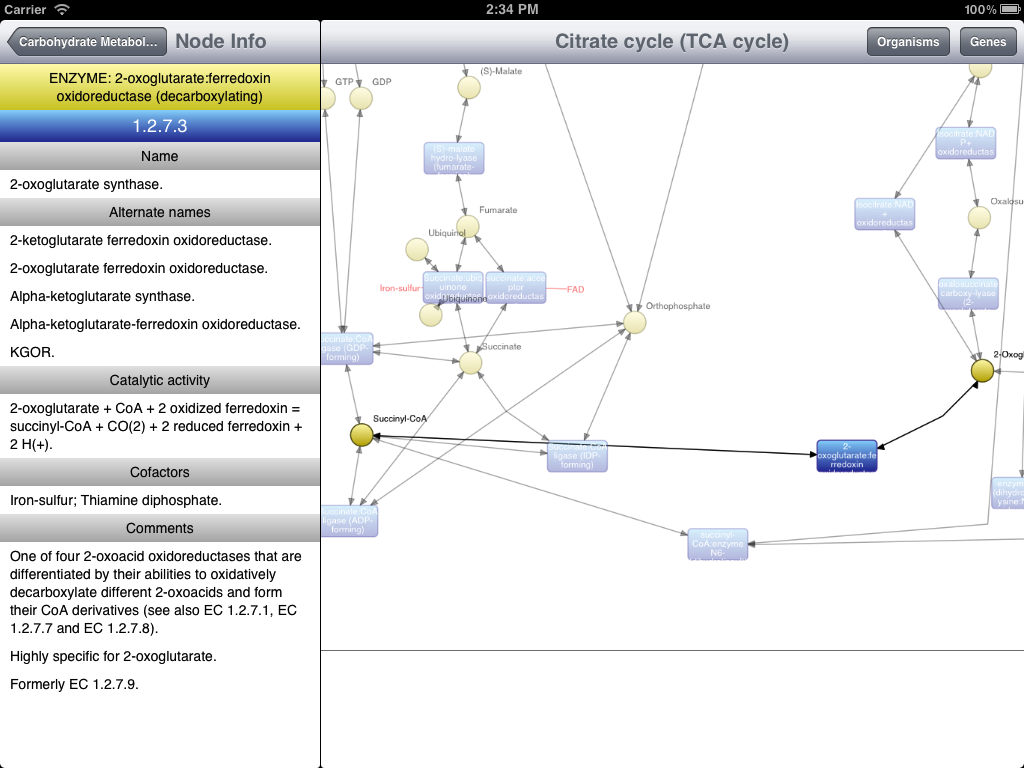
\includegraphics[width=3in]{kegg/figures/screenshot_selection_info}}
    \caption{\label{fig:kegg_screenshot_selection_info} Sidebar showing
    information from the ENZYME database for the reaction ``2-oxoglutarate
    synthase''}
\end{figure}
